\documentclass[a4paper]{extarticle}
\usepackage[utf8]{inputenc}
\usepackage[a4paper, margin=1in]{geometry}

\usepackage{amssymb}
\usepackage{amsmath}
\usepackage{enumitem}
\usepackage{tcolorbox}
\usepackage{fancyhdr}
\usepackage{graphicx}
\usepackage{float}

\setlength{\parindent}{0em}
\setlength{\parskip}{0.4em}

\definecolor{theoremblue}{RGB}{1, 73, 124}
\definecolor{corollaryblue}{RGB}{70, 143, 175}
\definecolor{exampleblue}{RGB}{137, 194, 217}

\newtcolorbox{tbox}{colback=theoremblue!20,colframe=theoremblue,
boxrule=0pt,arc=0pt,boxsep=2pt,left=2pt,right=2pt,leftrule=2pt}

\newtcolorbox{cbox}{colback=corollaryblue!20,colframe=corollaryblue,
boxrule=0pt,arc=0pt,boxsep=2pt,left=2pt,right=2pt,leftrule=2pt}

\newtcolorbox{ebox}{colback=exampleblue!20,colframe=exampleblue,
boxrule=0pt,arc=0pt,boxsep=2pt,left=2pt,right=2pt,leftrule=2pt}

\title{EnpRisk - Lecture Notes Week 3}
\author{Ruben Schenk, ruben.schenk@inf.ethz.ch}
\date{\today}

\pagestyle{fancy}
\fancyhf{}
\rhead{ruben.schenk@inf.ethz.ch}
\rfoot{Page \thepage}
\lhead{EnpRisk - Lecture Notes Week 3}

\begin{document}

\maketitle
\newpage

\subsubsection{How to Deal with Biases?}

We introduce different strategies on how to \textbf{deal with biases:}

\paragraph{Heuristics} Whend predictability is poor, inconsistency, based on unnoticed stimuli, is destructive of any predictive validity. Be consistent by using investment criteria, simple formulas, recipies or rules of thumb.

\paragraph{Example, consider an outside view} Prior to the use of any inside information, try to predict a totally independent base rate, e.g. "how many start-ups in this field survive the first three years?" Use this as your anchor and adjust this base rate according to information obtained during the due diligence.

\paragraph{Decorrelate error} Ask people's opinion independently of each other, wisdom of crowds versus groupt think, practice "constructive confrontation", avoid "cozy unanimity".

\paragraph{Sunk Cost} Be aware of the difficulty to take a loss. A new manager does not carry the same mental accounts and is therefore more able to ignore the sunk cost of past investments.

\paragraph{Validity of intuition} Intuition cannot be trusted in the absence of stable regualrities in the environment and in the absence of prolonged practice and learning.

\subsection{From the First Pitch to the Final Investment}

\subsubsection{NDA - Non-Disclosure Agreement}

If the introduction round is finished successfully a \textbf{Non-Disclosure Agreement (NDA)} is signed between the investors and the founders. This is a legal contract that outlines the use of confidential material, knowledge, and information that the parties wish to exchange.

Some common issues addressed in an NDA:

\begin{itemize}
    \item The definition of what is confidential (e.g. trade secrets, upublished patent applications, vendor lists, customer lists, financial information, business strategies, etc.)
    \item Exclusions (e.g. information independently obtained)
    \item The time period of confidentiality
    \item Description of what must be done with the confidential material upon agreement ending (duty to return or destroy)
\end{itemize}

After the NDA is signed by both parties, access is given to the data room.

\subsubsection{Term Sheet / Letter of Intent}

After a first check of the data room, the investors will produce a term sheet or LOI, which:

\begin{itemize}
    \item Outlines an agreement that two or more parties expect to make.
    \item Term Sheet and LOI are very similar in content, but TS is structured as a listen, often in table format, whereas LOI is in the form of a letter.
    \item Written before the execution of a formal and binding contract, most of the lsited agreements are \textit{not legally binding.}
\end{itemize}

The topics included are:

\begin{itemize}
    \item Valuation of the company
    \item Amount of investment
    \item Use of proceeds
    \item Cap table
    \item Share preference
    \item Governance (board composition and chair, voting rights, etc.)
    \item Investor commitment (lock up period)
    \item Management commitment
\end{itemize}

\subsubsection{Exclusivity}

This is a binding clause of the LOI or TS. Caveat: Transfers a lot of control to the investor, he will be the only party taking the next step in the process, he can take advantage of the "sunk cost effect", often exclusivity periods are extended. The investor can put you under pressure, test your tenacity and patience, try to decrease the valuation of the company, etc.

\textit{When you give exclusivity, you cancel out any competition for the investor, this will make him dominant.}

\subsubsection{Due Diligence}

After the TS and/or LOI are signed, the \textbf{Due Diligence} process is started. This is supposed to take up to six weeks, in reality, it will turn out to be many months. Now, the external advisors enter the arena:

\begin{itemize}
    \item Business lawyers will examine all the contracts in the data room
    \item IP lawyers will study the strengths of the patents of the company and the "freedom to operate"
    \item An external auditor will validate the accounting, financial statements, balance sheets, and taxes
    \item A technological consultant may analyze the product developement and the strength and relevance of the technology with respects to other solutions
\end{itemize}

The investors themselves will:

\begin{itemize}
    \item Do reference checks of clients, founders, key personnel
    \item Analyze the commercial viability of the product and the sales process and tools
    \item Study the quality of the sales pipeline
    \item Based on that will make their own forecast of future sales
    \item And a forecast of future cashflows
\end{itemize}

Based on the results of the due diligence, the investors will challenge the business plan. This will allow them to:

\begin{itemize}
    \item Create base-case and worst-case scenarios of cash burn
    \item Check the investment amount and the use proceeds with respect to these scenarios
    \item Access the risk of their investment
    \item Set goals and milestones for the management
    \item Make their own valuation of the company
\end{itemize}

\subsection{Introduction to Company Valuation}

\subsubsection{Overview}

We will give three approaches towards valuations:

\begin{itemize}
    \item \textit{Balance sheet:} Static, i.e. a snapshot: Equity = Assets - Liabilities
    \item \textit{P\&L:} Relative values by using multiple metrics from the Profit \& Loss account
    \item \textit{Discounted cash flow:} Absolute values by using the cash flows that will be generated by the business to calculate the Net Present Value of the business - like in the valuation of a bond.
\end{itemize}

Before we start, let us first explain the difference ebtween EV and Equity:

\begin{itemize}
    \item \textbf{Enterprise Value (EV)} is the price to acquire the whole company, the shares, the debt but also receiving the cash
    \item \textbf{Equity Value} is the price to acquire only the shares of a company.
\end{itemize}

In other words: Enterprise Value (EV) = Equity + Debt - Cash

\subsubsection{Balance Sheet and Leverage}

A \textbf{Balance Sheet} is of the following form:

\begin{figure}[H]
    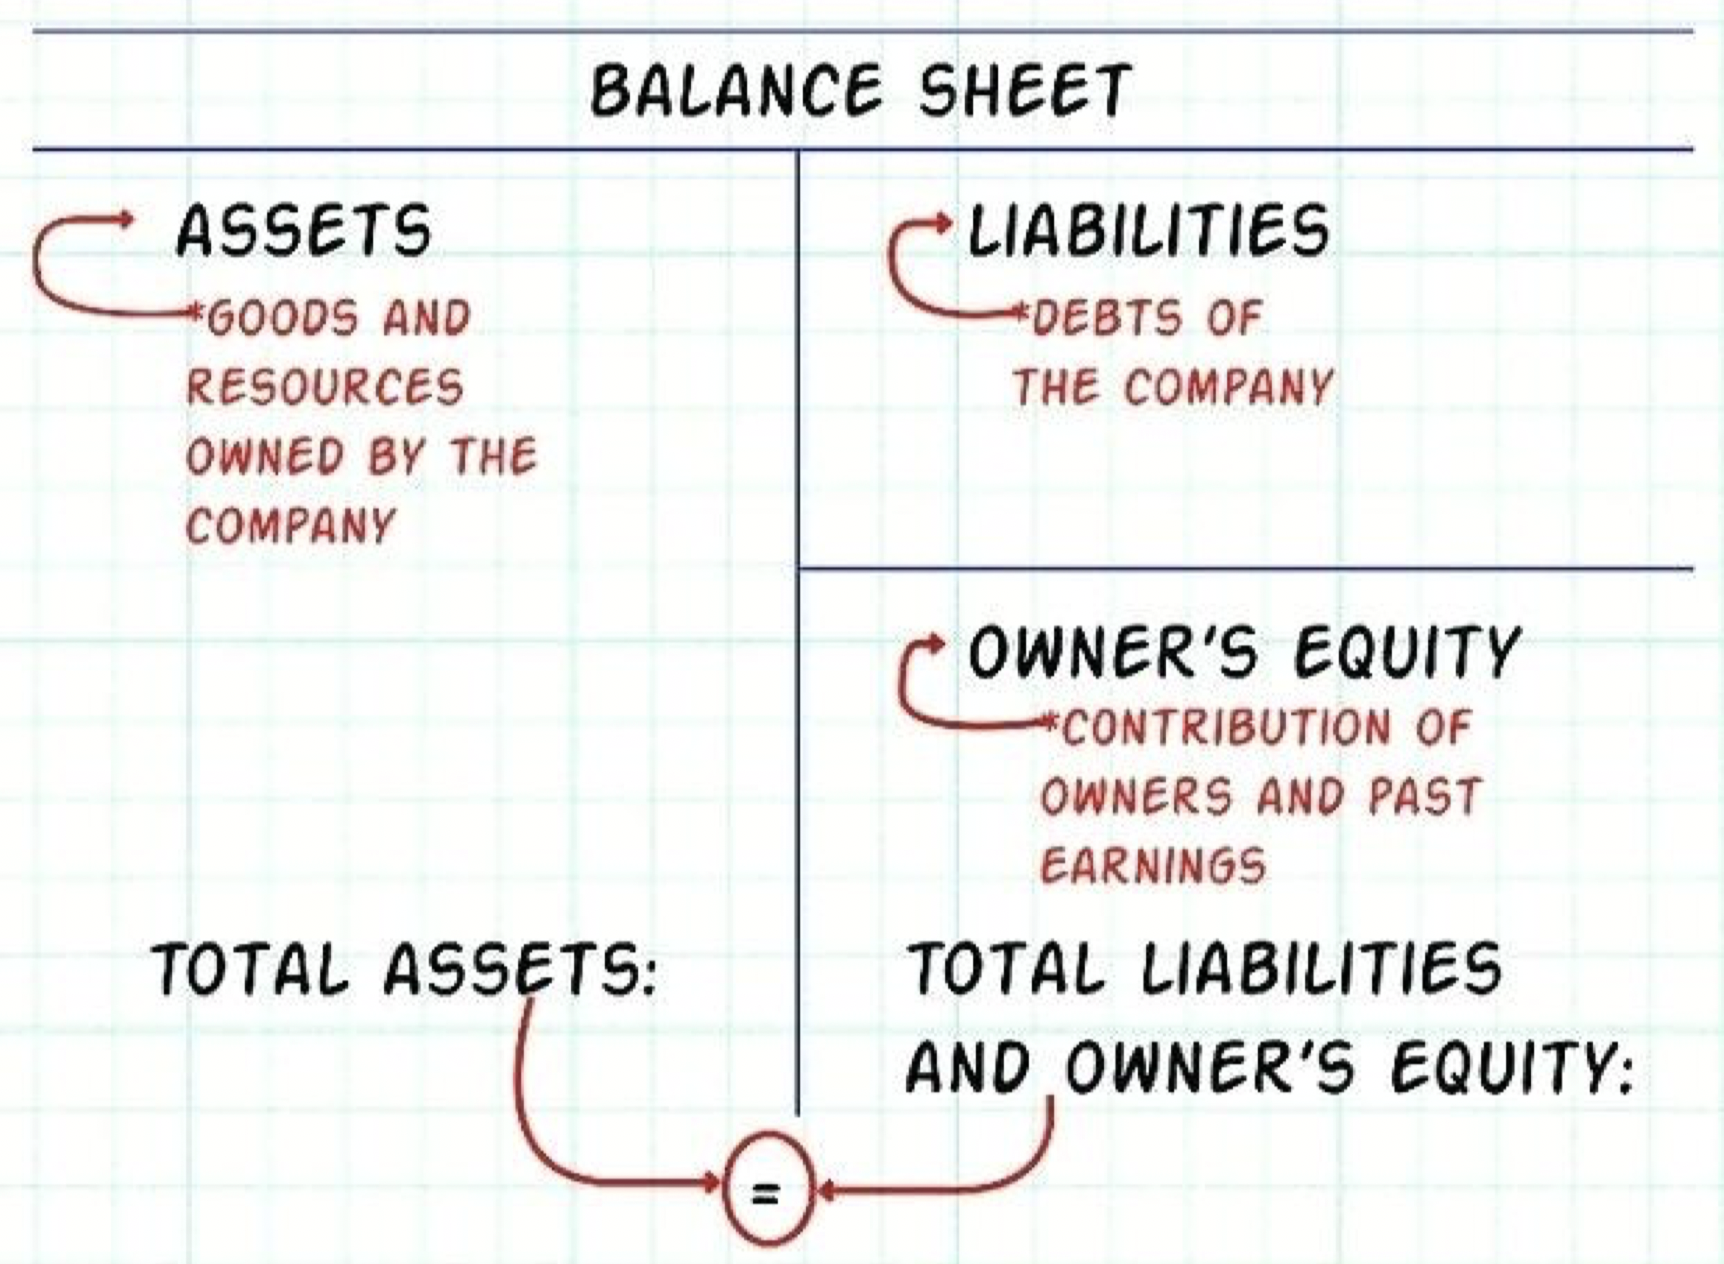
\includegraphics[width=11cm]{../images/EnpRisk_Fig3-1}
    \centering
\end{figure}

\begin{ebox}
    \textbf{Example:} Assume we start a taxi business:

    \begin{itemize}
        \item We buy 5 Tesla Model 3 at a price of 40 kCHF each
        \item Our total investment is 200 kCHF
        \item To set up a LLC in Switzerland we need to pay up, personally, a minimu share capital of 20 kCHF
        \item We found a bank that was kind enough to provide us with a 5 year loan of 200 kCHF to buy the cars
    \end{itemize}

    Our initial balance sheet will look like this:

    \begin{figure}[H]
        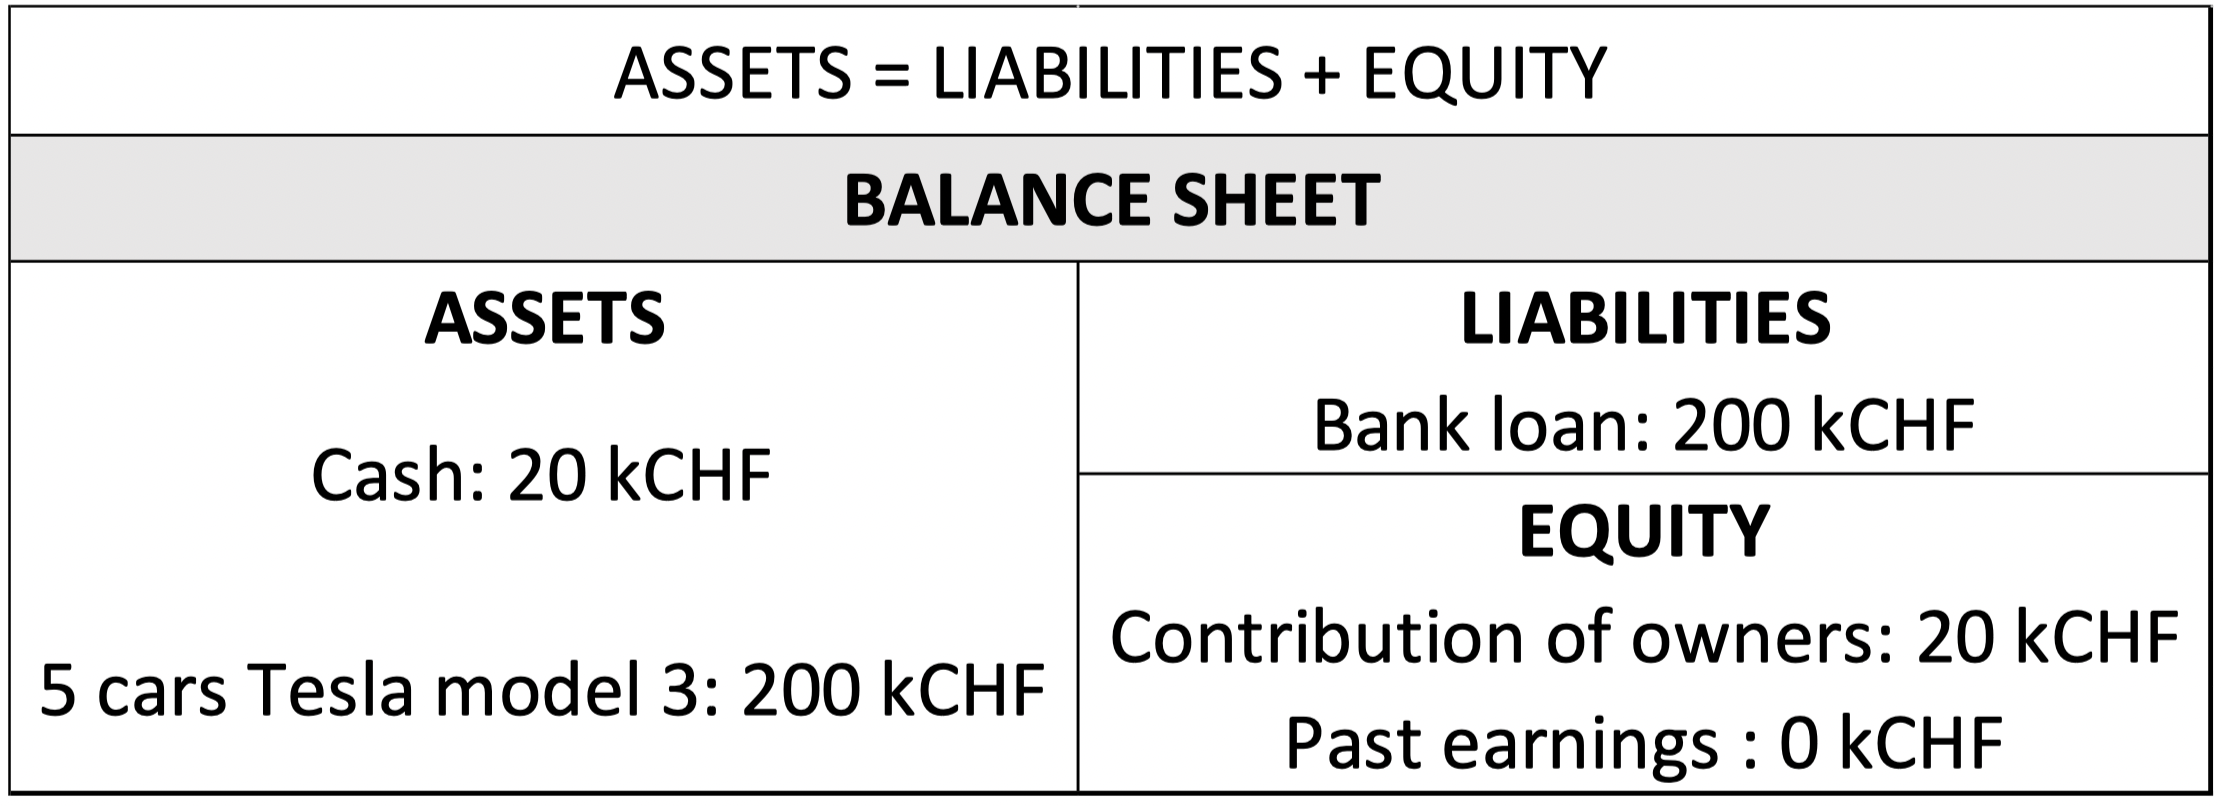
\includegraphics[width=9cm]{../images/EnpRisk_Fig3-2}
        \centering
    \end{figure}

    The balance sheet changes with the business, after one year it may look like this:

    \begin{figure}[H]
        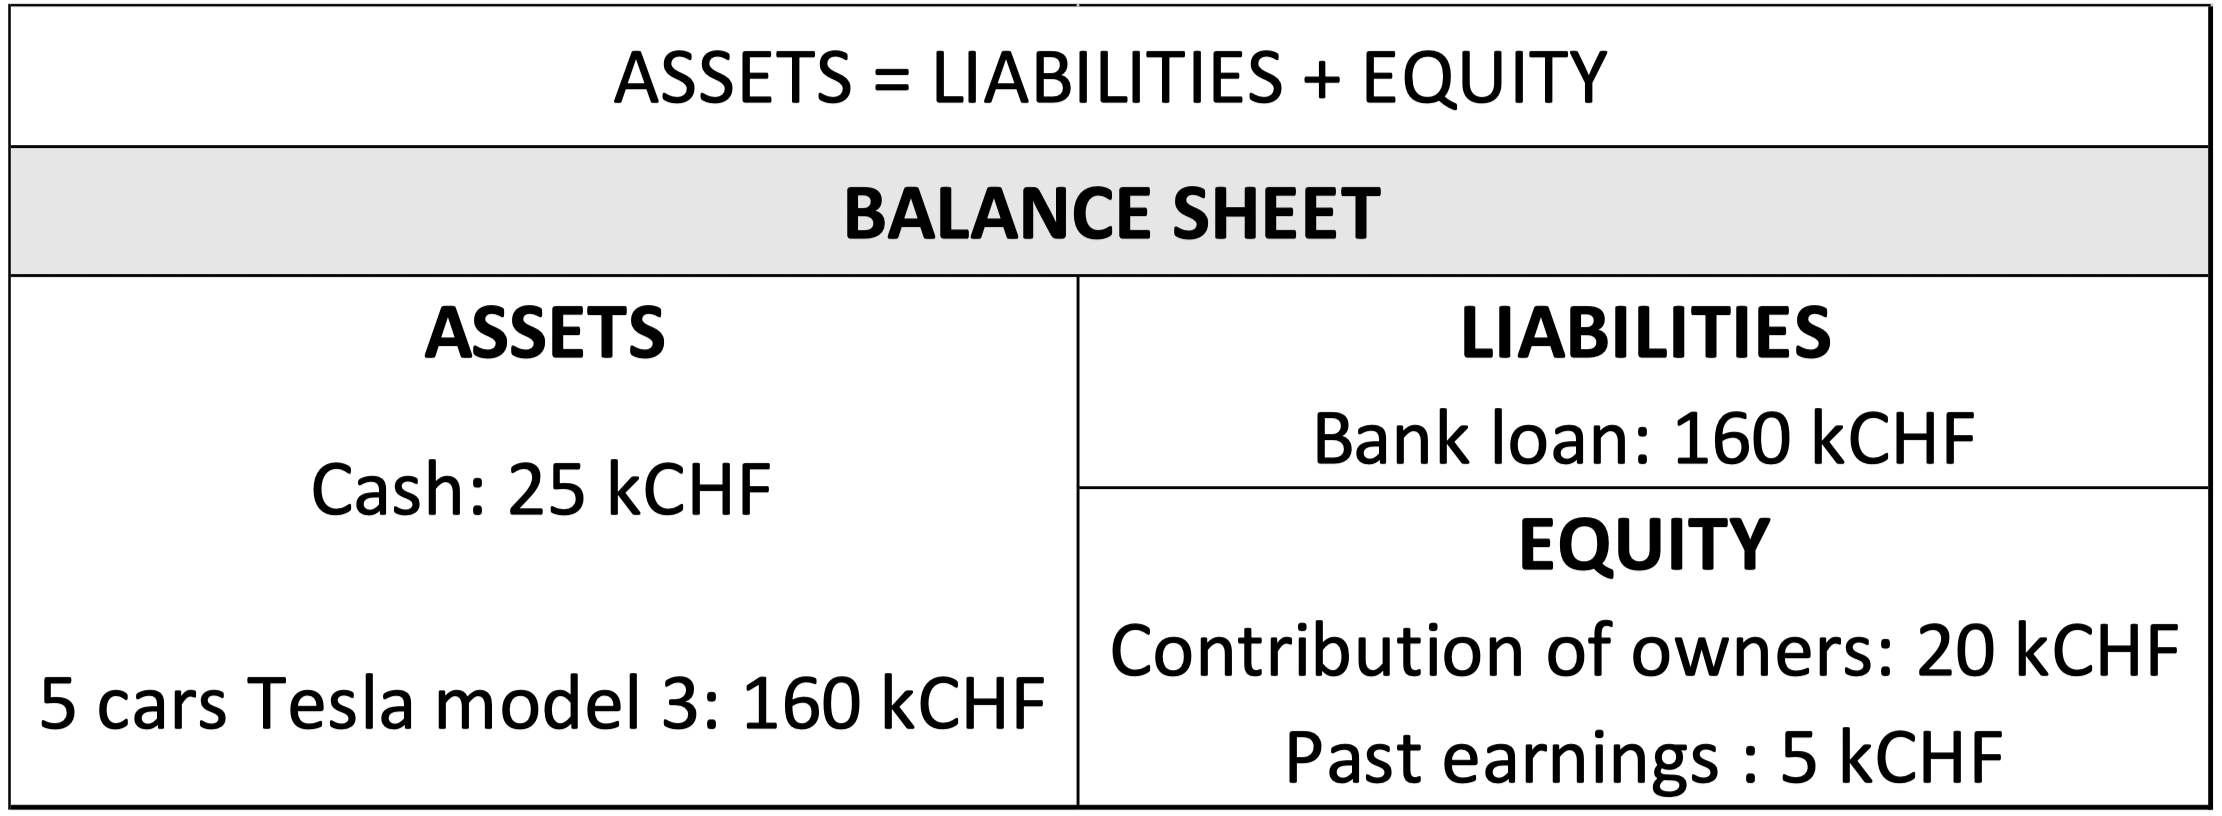
\includegraphics[width=9cm]{../images/EnpRisk_Fig3-3}
        \centering
    \end{figure}

    \begin{itemize}
        \item You made a profit of 5 kCHF, you paid down 20\% of the bank loan and the cars lost 20\% in value
        \item Your \textbf{Return on Equity (ROE)} is 25\%, you did very well! But your \textbf{financial leverage (Debt-to-Equity)} is 6.4 (160/25), which is very high
        \item Now the value of the company is 25 kCHF
    \end{itemize}

    If we do the same calculations, but started with 10 cars, we get the following balance sheet after 1 year:

    \begin{figure}[H]
        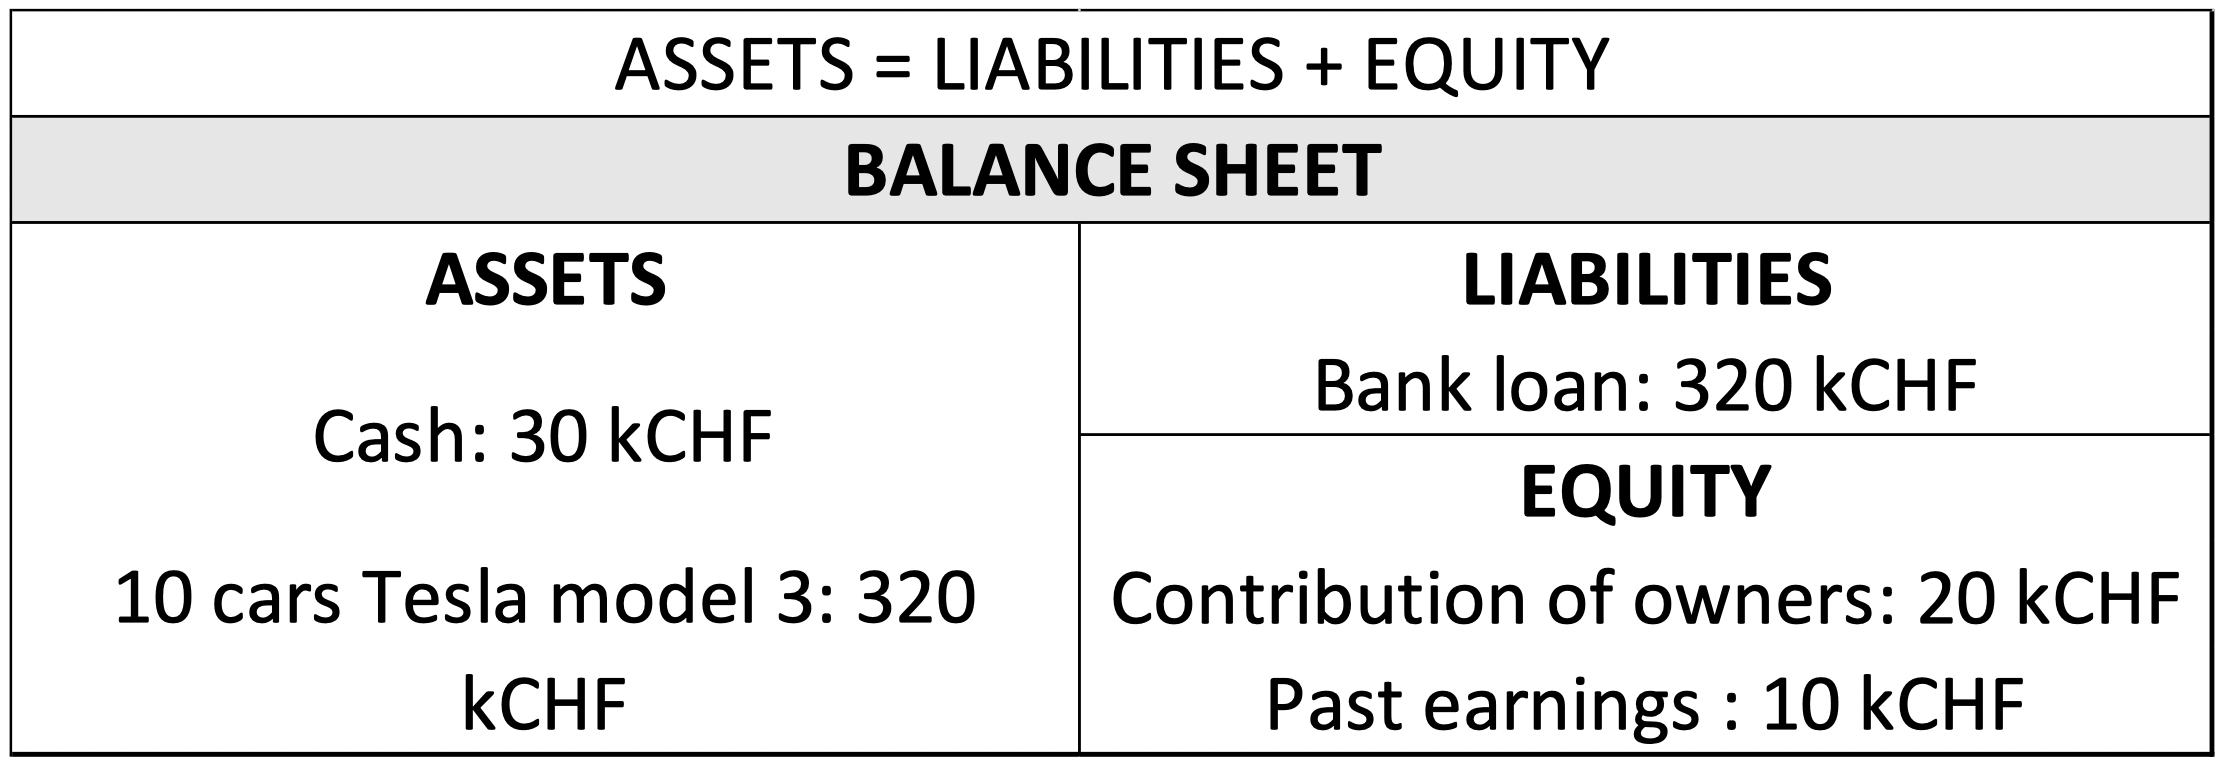
\includegraphics[width=9cm]{../images/EnpRisk_Fig3-4}
        \centering
    \end{figure}

    \begin{itemize}
        \item After one year, the profit could have been around 10 kCHF, you paid down 20\% of the bank loan, and the cars lost 20\% in value
        \item Now the ROE is 50\% and the financial leverage is 10.7 (320/30)
        \item \textit{You made 10x more money with the same investment, but the risk is much higher!}
    \end{itemize}
\end{ebox}

We have seen that leverage increases your risk proportionally. The larger your business is, the higher your losses can be. If you increase your business with debt, and without increasing the equity buffer proportionally, you will have a higher ROE but als a much higher \textit{risk of insolvency} (i.e. not being able to service the larger amount of debt).

When you continue accumulating losses, after some time you will have consumed your full equity buffer. Because of the cash you burn, your debts become higher than your assets, your company has so-called negative equity. Often that is a sign of future insolvency.

\subsubsection{Banking}

For our taxi business, the losses may come from operating the business. These losses may eat up the equity buffer and lead to insolvency and bankruptcy. There is no substantial risk from assets depreciating unexpectantly.

This is quite different for a bank. A bank can also have operational losses eating up its equity, but in addition, there may be large market depreciation of its assets during a financial crisis.

The leverage ratios of the five major investment banks were as high as 40 to 1 (2007). This means that a \textit{mere drop of 2.5\% in the value of their assets would wipe out entirely their equity buffer} and basically reduce their stock prices, which were soraing high, to zero.

The banking system is a closely knitted system. When a bank A collapses, this may lead to asset depreciations for bank B. As a result, also B gets in trouble. When banks get in trouble, they no longer provide loans to companies. As a result, the whole economic systems gets infected.

\textbf{Too much leverage in the system may make it very vulnerable and susceptible to systemic shocks.}

\subsubsection{P\&L - Profit and Loss}

Lets go back to out taxi business and introduce several different metrics:

\begin{figure}[H]
    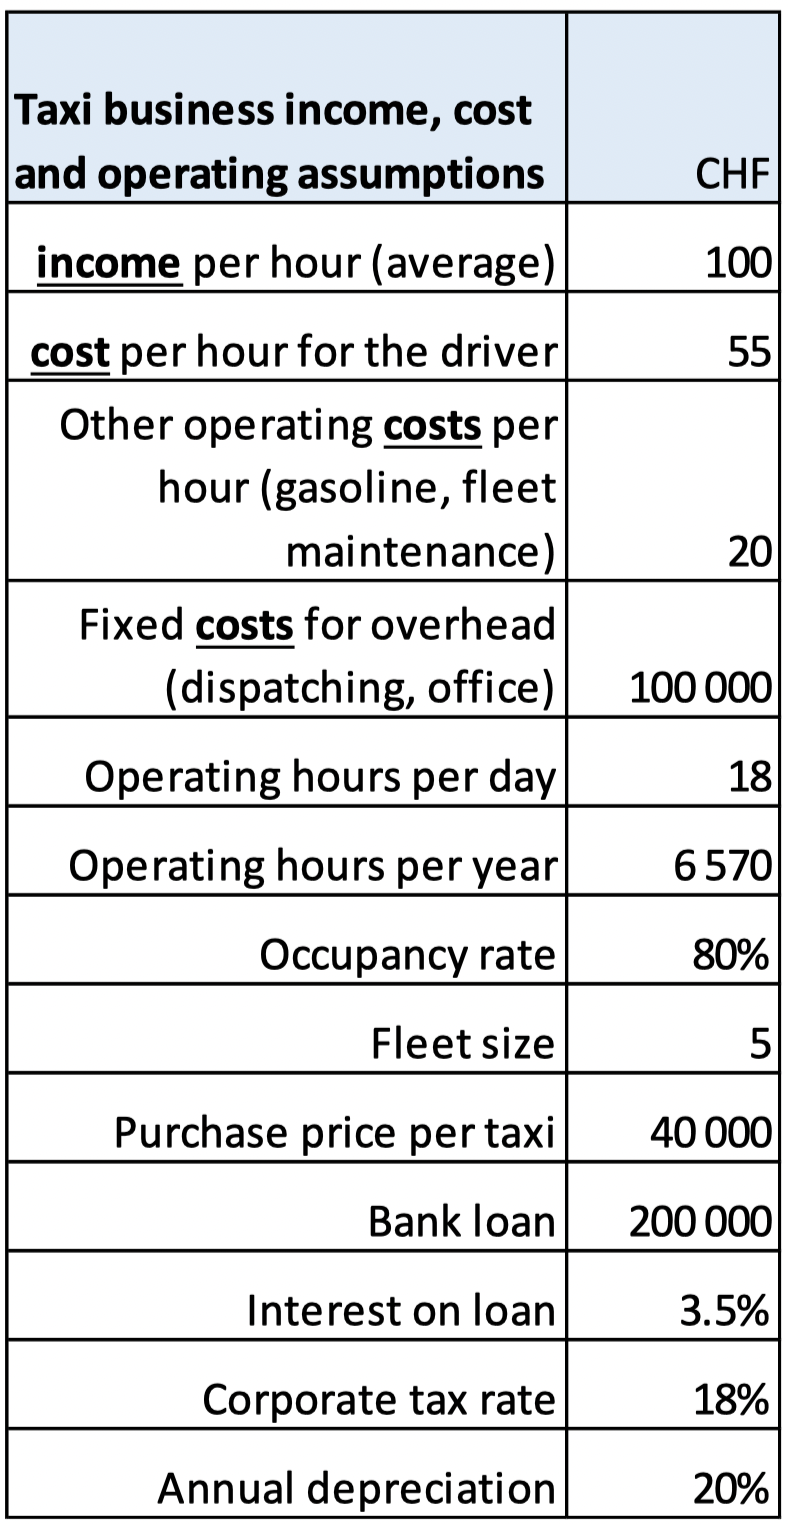
\includegraphics[width=5cm]{../images/EnpRisk_Fig3-5}
    \centering
\end{figure}

\begin{itemize}
    \item \textbf{Revenues (sales)} = income per hour * operating hours per year * occupancy rate * fleet size = 2'628'000 CHF (per year)
    \item \textbf{Cost of goods sold (COGS)} = cost of the material and the labor directly used to rund the business = operating hours per year * fleet size * (cost per hour for the driver + operating costs * occupancy rate) = - 2'332'350 CHF
    \item \textbf{Gross Margin} = Revenue - COGS = 295'650 CHF = 11.3\%
    \item \textbf{Operating Expenses (OPEX)} = the remaining costs that are not included in COGS = - 140'000 CHF
    \item \textbf{Earnings Before Interest and Taxes (EBIT)} = Gross Margin - OPEX = 155'650 CHF = 5.9\%
    \item \textbf{Earnings Before Interest, Taxes, Depreciation and Amortization (EBITDA)} = EBIT + D\&A = 195'650 CHF = 7.4\%
    \item \textbf{Earnings Before Taxes (EBT)} = EBIT - Interests paid = 148'650 CHF
    \item \textbf{Taxes} = - 26'757 CHF
    \item \textbf{Net Profit} = EBIT - Interests paid - Taxes = 121'893 CHF = 4.6\%
\end{itemize}

Finally, our P\&L looks as follows:

\begin{figure}[H]
    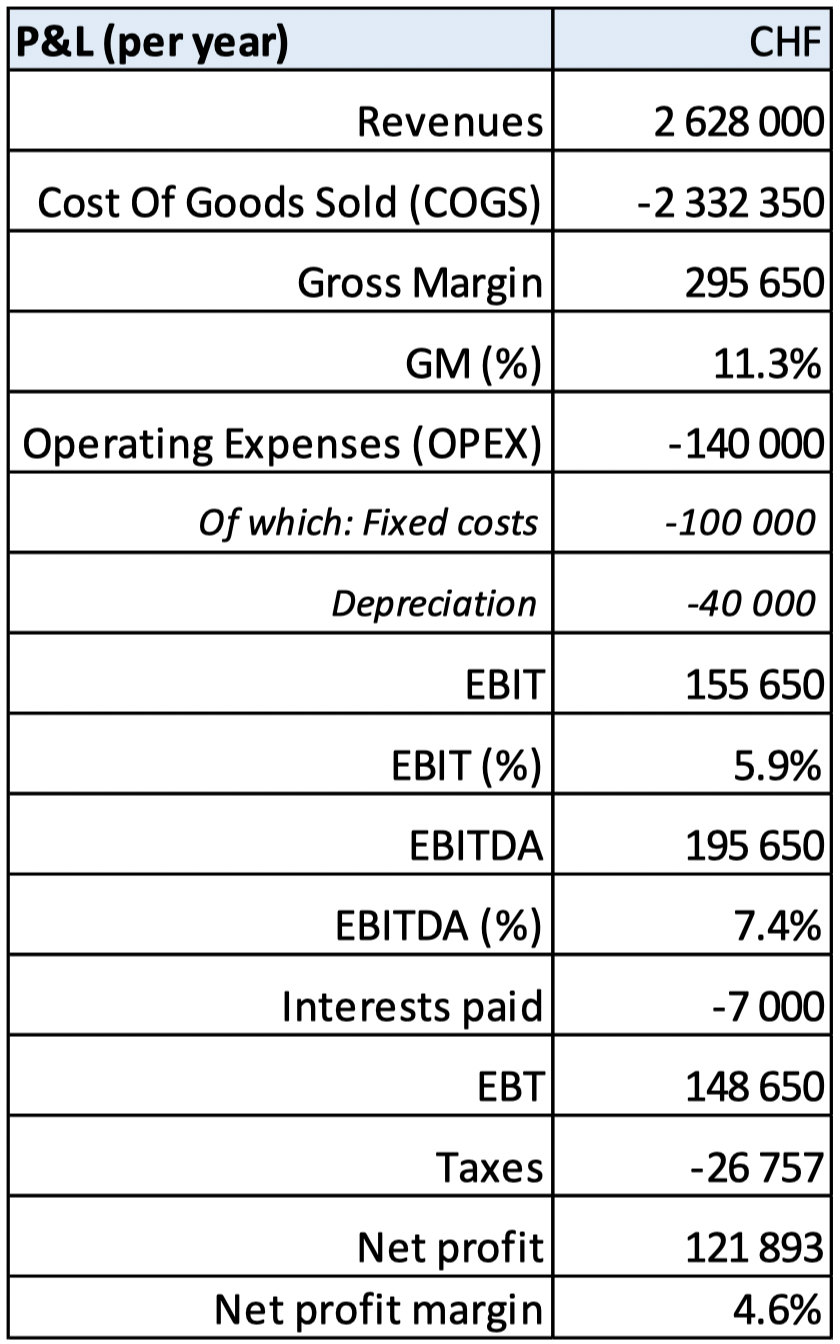
\includegraphics[width=5cm]{../images/EnpRisk_Fig3-6}
    \centering
\end{figure}

\end{document}